% CS461 final report. Build from this folder with:  latexmk -pdf report.tex
% Figures come straight from ../../results/figures, so regenerated plots appear automatically.

\documentclass[10pt,a4paper]{article}

% --- Page and fonts -------------------------------------------------------
\usepackage[margin=2cm]{geometry}   % narrower margins: the brief allows 5 pages
\usepackage{lmodern}                % scalable Latin Modern fonts (load before fontenc, or MiKTeX makes bitmap fonts)
\usepackage[T1]{fontenc}            % proper accented characters and hyphenation
\usepackage[utf8]{inputenc}         % the .tex file itself is UTF-8
\usepackage{microtype}              % subtle spacing tweaks: fewer bad line breaks

% --- Content packages -----------------------------------------------------
\usepackage{graphicx}               % \includegraphics
\usepackage{booktabs}               % clean tables: \toprule \midrule \bottomrule
\usepackage{subcaption}             % two figures side by side, each with its own caption; also \captionof
\usepackage{enumitem}               % compact lists
\setlist{nosep, leftmargin=*}
\usepackage[hidelinks]{hyperref}    % clickable references and URLs, no coloured boxes
\usepackage{xcolor}
\usepackage{placeins}               % \FloatBarrier: keep tables/figures inside their own section

\graphicspath{{../../results/figures/}}
% LaTeX's defaults keep figures to at most 70% of a page top and need 20% text per page,
% which left half-empty pages; a figure-heavy short report needs looser limits.
\renewcommand{\topfraction}{0.9}
\renewcommand{\bottomfraction}{0.8}
\renewcommand{\textfraction}{0.07}
\renewcommand{\floatpagefraction}{0.75}
\setlength{\parskip}{3pt}

\title{Real-time ASL Fingerspelling Practice with Hand Landmarks:\\
       an MLP vs CNN Comparison on a Real Webcam}
% Real name and student ID live in author.tex, which is gitignored (the repo is public).
% Create it next to this file with one line:  \newcommand{\studentline}{Your Name, 6xxxxxxxxx}
\IfFileExists{author.tex}{\input{author.tex}}{\newcommand{\studentline}{Student name, ID}}
\author{CS461 Neural Networks and Deep Learning --- Final Project\\
        \small \studentline \quad (\url{https://github.com/tecchuuu/asl-fingerspelling-trainer})}
\date{November 2026}

\begin{document}
\maketitle

% =========================================================================
\section{Problem and business value}

Learning to fingerspell takes a lot of repetitive drill: a learner forms a letter, an
instructor checks it, and they repeat. That drill uses instructor time that would be better
spent on teaching. This project builds a \textbf{practice tool, not a translator}: a web app
that watches the learner's hand through a webcam and checks each letter in real time, so drill
can happen without an instructor present.

The scope is the \textbf{ASL alphabet} (no public Thai Sign Language dataset exists) and its
\textbf{24 static letters}; J and Z require motion. The research question is whether
\textbf{hand landmarks beat raw images}, in accuracy, size and speed, and above all on a
\emph{real webcam} rather than the dataset's own test split. Targets from the proposal: macro
F1 $\geq 90\%$ on the dataset test set, $\geq 80\%$ on a live webcam test, and $\leq 33$\,ms
processing per frame.

% =========================================================================
\section{Data}

The ASL Alphabet dataset~\cite{asl} has 3,000 photos per letter (72,000 for the 24 letters),
recorded by few signers in one room. MediaPipe Hand Landmarker~\cite{mediapipe} extracts 21
3-D landmarks per hand; it found a hand in 77.3\% of images on the first pass. Most failures
were backlit (a dark hand against a bright window). Retrying the failures after brightening
recovered 2.1\% with CLAHE but \textbf{43.0\% with gamma correction} ($\gamma=0.5$), giving
\textbf{62,704 images (87.1\%)}, 1,788 (N) to 2,977 (F) per letter. Each recovered sample is
flagged. The \texttt{nothing} class was dropped: it has no hand, so ``no hand detected'' plays
its role in the app.

\textbf{Data audit.} Checking the photos against an ASL dictionary showed that the dataset's
\textbf{T is not standard ASL} (thumb sideways instead of tucked between the index and middle
fingers). Signing the correct T, the final model accepted it \textbf{0 of 5 times} (reading it
as A). K and P are minor variants that still generalise (4/5 and 5/5 accepted).

% =========================================================================
\section{Method}

\textbf{Pipeline.} Webcam frame $\rightarrow$ MediaPipe (21 landmarks) $\rightarrow$
normalisation $\rightarrow$ classifier $\rightarrow$ confidence gate $\rightarrow$ typed letter.

\textbf{Normalisation.} The $x$ and $z$ coordinates are multiplied by the frame's aspect ratio
(MediaPipe normalises $x$ and $y$ by different image sides), the wrist is subtracted, and
everything is divided by the palm length (wrist to middle-finger knuckle), which unlike the
bounding box does not change with finger pose. Rotation is deliberately \emph{not} normalised:
orientation distinguishes letters (P/Q point down, G/H sideways). Without any training, a
nearest-centroid classifier improves from \textbf{50.4\% to 85.4\%} with this normalisation.

\textbf{Split and augmentation.} Frames are numbered in recording order and neighbours are
near-duplicates (consecutive frames are $\sim$4$\times$ closer in landmark space than random
pairs). Whole blocks of 100 frames therefore go to one split, 70/15/15 per letter (44,989 /
9,132 / 8,583). A 1-nearest-neighbour classifier scores 98.8\% on a random split but 96.4\% on
the block split, evidence that a random split leaks. Training data is doubled with mirrored
copies ($x \rightarrow -x$) so left hands are covered.

\textbf{Models.} \emph{Model B (main):} an MLP, 63 inputs $\rightarrow$ 256 $\rightarrow$ 128
$\rightarrow$ 24, ReLU, dropout 0.3, 52,376 parameters. \emph{Model A (baseline):} a CNN on
64$\times$64 hand crops cut around the landmarks, three Conv--BatchNorm--ReLU--MaxPool blocks
(32/64/128 channels), global average pooling, 96,792 parameters. Both use the same split and
the same final training settings, so the comparison isolates the \emph{input}: landmarks
versus pixels.

\textbf{From frames to letters.} A gate types a letter once the same prediction wins 10
consecutive frames with confidence $\geq 0.8$, does not repeat it while it is held, and types
it again when the hand slides sideways by $\geq 0.6$ palm lengths (how signers mark double
letters). Because a closed-set classifier must label \emph{every} hand, a resting open hand was
typed as F; a 25th class, \emph{other} (my recordings of non-letter hand poses), plus a rule
that a thumb--index pinch cannot be ``other'' cut resting hands typing a letter from
\textbf{69\% to 7.5\%} of frames.

% =========================================================================
\section{Model Tuning \& Optimization}

The \textbf{baseline} is the first, untuned MLP (Adam, learning rate $10^{-3}$, batch 32, fixed
rate, dropout 0.3, early-stopping patience 5): validation macro F1 96.45\%, validation loss
0.1175. All runs use seed 42, the same split and early stopping on validation loss; the test
set was not used for any choice.

\textbf{Optimizers and batch size.} Adam~\cite{adam} and SGD with momentum 0.9 (learning rate
$10^{-2}$) were each run with batch 32 and 64 (Table~\ref{tab:opt},
Figure~\ref{fig:tuning}a). All four end within 0.25 F1 points, which is about the size of
run-to-run noise, so neither optimizer is more accurate here. The difference is
\textbf{convergence}: Adam reaches $\sim$94\% F1 by epoch 2--3, while SGD with batch 64 needs
$\sim$8 epochs for that and 30 to reach its best, as expected from Adam's per-weight step sizes.
Batch 64 gives visibly smoother validation curves than batch 32.

\begin{table}[ht]
\centering\small
\begin{tabular}{llcccc}
\toprule
Optimizer & Batch & Val F1 & Val loss & Best epoch & Time \\
\midrule
Adam ($10^{-3}$) & 32 & 96.45\% & 0.1175 & 9 & 108\,s \\
\textbf{Adam ($10^{-3}$)} & \textbf{64} & \textbf{96.60\%} & \textbf{0.1133} & 20 & 87\,s \\
SGD + momentum ($10^{-2}$) & 32 & 96.37\% & 0.1204 & 15 & 88\,s \\
SGD + momentum ($10^{-2}$) & 64 & 96.44\% & 0.1161 & 30 & 101\,s \\
\midrule
Adam, batch 64 + LR schedule & & \textbf{96.81\%} & \textbf{0.1013} & 44 & 157\,s \\
\quad + dropout 0.5 (instead of 0.3) & & 96.51\% & 0.1165 & 45 & 158\,s \\
\bottomrule
\end{tabular}
\caption{Tuning runs on the MLP (validation set). Top: optimizer $\times$ batch size. Bottom:
follow-ups on the winner, with early-stopping patience 8.}
\label{tab:opt}
\end{table}

\textbf{Learning-rate schedule.} The fixed-rate curves kept bouncing after epoch $\sim$10
(validation loss 0.11--0.16), a sign of steps too large to settle. ReduceLROnPlateau (halve the
rate after 2 epochs without improvement) lowered validation loss by \textbf{11\%}
(0.1133 $\rightarrow$ 0.1013) and removed the late spikes (Figure~\ref{fig:tuning}b). A lesson
from the first attempt: with early-stopping patience 5, training stopped one epoch after the
first rate cut, before it could help; the early-stopping patience must exceed the scheduler's.
Both runs were repeated with patience 8. With a fixed seed the two runs are identical until the
first rate cut, so the gain comes from the schedule alone.

\textbf{Regularisation.} With the schedule, training loss fell to 0.034 against 0.101 on
validation, so stronger dropout looked worth trying. Dropout 0.5 made both worse (training loss
rose to 0.078): dropping half the units of a small 256/128 network underfits. Dropout 0.3 was
kept, together with early stopping.

\textbf{Before $\rightarrow$ after.} Validation F1 96.45\% $\rightarrow$ \textbf{96.81\%};
validation loss 0.1175 $\rightarrow$ \textbf{0.1013} ($-14\%$). Tuning mainly improved
convergence and stability; the remaining errors come from the data (M/N, Q/P), not the
optimizer. The CNN was trained once with the final MLP settings (236\,s per epoch on CPU,
2.5\,h in total).

\begin{figure}[ht]
\centering
\begin{subfigure}{0.8\textwidth}
  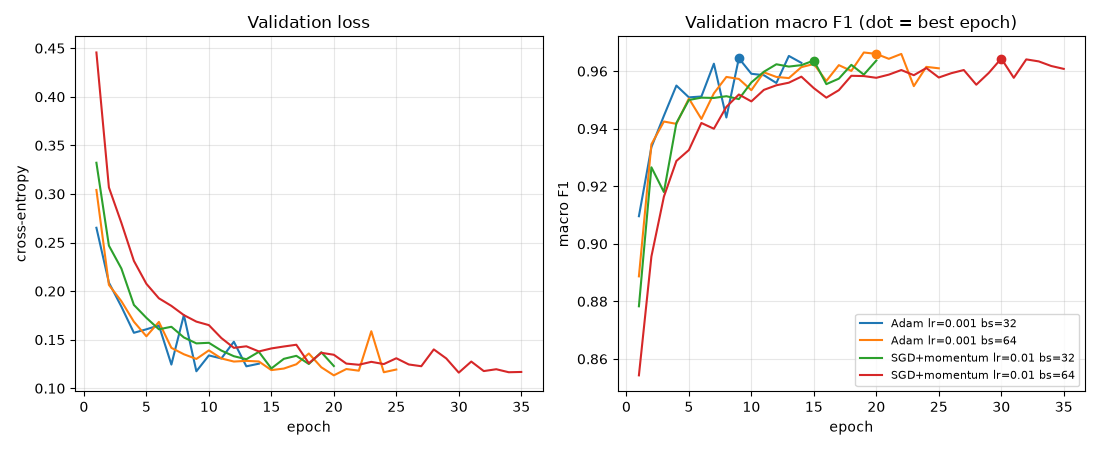
\includegraphics[width=\linewidth]{optimizer_comparison.png}
  \caption{Adam vs SGD+momentum, batch 32 vs 64.}
\end{subfigure}\\[6pt]
\begin{subfigure}{0.8\textwidth}
  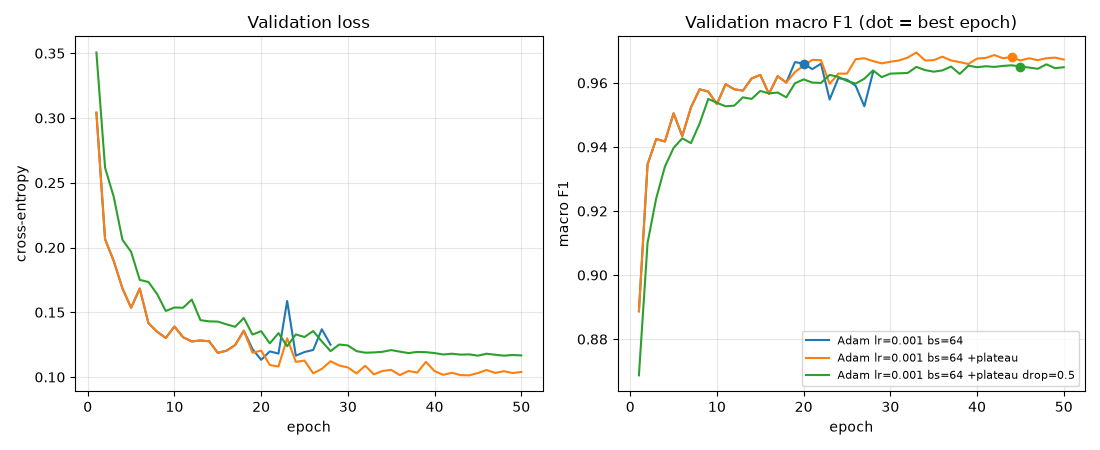
\includegraphics[width=\linewidth]{schedule_dropout.png}
  \caption{Fixed rate vs LR schedule; dropout 0.3 vs 0.5.}
\end{subfigure}
\caption{Validation loss (left) and macro F1 (right) per epoch for the tuning runs.}
\label{fig:tuning}
\end{figure}

% =========================================================================
\section{Results}

\textbf{Dataset test set} (8,583 samples, evaluated once on the final models): the MLP reaches
\textbf{98.1\%} macro F1 and the CNN 96.0\%, both above the 90\% target. The MLP has half the
parameters and is 20$\times$ faster per sample (0.07 vs 1.43\,ms). The models fail on different
letters: the MLP on M/N (thumb hidden under the fingers, so MediaPipe must guess hidden joints),
the CNN on H$\leftrightarrow$G (two stacked fingers look like one in a 64$\times$64 crop).

\textbf{Real webcam.} I recorded my own test set before looking at any webcam results: 24
letters $\times$ 3 captures per session, in three conditions, 216 samples in total, never used
for training. Table~\ref{tab:webcam} and Figure~\ref{fig:webcam} show the central result:
\textbf{on the dataset the two models are 2 points apart; on a real webcam they are about 80
points apart.} The CNN learned the appearance of one signer's room and collapses to chance level
in a dark room (4.2\% accuracy, $1/24$), while the landmark MLP stays above the 80\% target in
every condition. The CNN's 96\% on the dataset is not a training failure: the same scoring code
gives it 97.7\% on dataset crops.

\begin{figure}[ht]
\centering
\begin{minipage}[c]{0.43\textwidth}
  \centering\small
  \begin{tabular}{@{}lccc@{}}
  \toprule
  Condition & $n$ & MLP & CNN \\
  \midrule
  Room light, right hand & 72 & \textbf{98.6\%} & 17.4\% \\
  Room light, left hand  & 72 & \textbf{91.3\%} & 18.1\% \\
  Dark, right hand       & 72 & \textbf{87.0\%} & 0.8\% \\
  \midrule
  All webcam   & 216 & \textbf{93.1\%} & 16.0\% \\
  \emph{Dataset test} & 8,583 & \emph{98.1\%} & \emph{96.0\%} \\
  \bottomrule
  \end{tabular}
  \captionof{table}{Macro F1, webcam (one signer) vs dataset test, 24-letter models.}
  \label{tab:webcam}
\end{minipage}\hfill
\begin{minipage}[c]{0.55\textwidth}
  \centering
  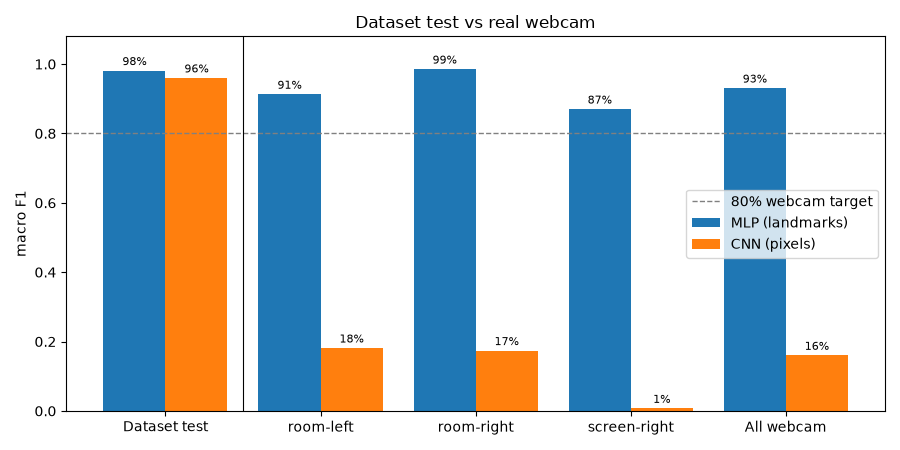
\includegraphics[width=\linewidth]{webcam_vs_dataset.png}
  \caption{Dataset test vs real webcam per session; dashed line: 80\% target.}
  \label{fig:webcam}
\end{minipage}
\end{figure}

On the webcam the MLP's main weakness is Q$\rightarrow$P (6 of 9 Q's): both point down, and my
camera is mounted high, looking down, an angle the dataset does not have. The left hand costs
7 points (mirroring mostly works) and darkness 12. \textbf{Speed:} the full pipeline takes
\textbf{10.8\,ms per frame} (median; 13.2\,ms at the 95th percentile) on a laptop CPU, against
a 33\,ms target; MediaPipe is 98\% of that and the MLP 0.25\,ms. \textbf{Browser vs Python:}
the web app runs MediaPipe in the browser; on 26 frames of all 24 letters it gave the same
letter as Python every time, with landmarks a median 3\,px apart.

\FloatBarrier  % results tables and figures must appear before the next section
% =========================================================================
\section{Application and business results}

The web app (React + FastAPI) has a Learn page, Practice by category, an Exam mode scored on the
first try, free spelling, a learner progress page, and a trainer dashboard. Every attempt is
logged to SQLite. To illustrate the trainer view, I \textbf{simulated} a class of 20 learners over
4 weeks: learner behaviour (skill, practice frequency, learning rate) is assumed, but each
letter's recognition rate is \emph{measured} from the real app on my webcam test. In this
simulation learners master a median of 19/24 letters and exam scores rise from 77\% to 83\%.
The letters the class gets stuck on separate two problems a trainer would handle differently:
\textbf{model limits} (O, Q, S, which the app often rejects) and \textbf{content gaps} (T and X,
practised only $\sim$8--10 times per learner because they appear in no practice words).
Estimating instructor time as practice hours divided by the drill-group size, the simulated
class's 43.9 practice hours replace about 4.4 instructor hours for a group of 10 (about
THB\,1,756 at an assumed THB\,400/h). All of these inputs are assumptions, adjustable on the
dashboard.

% =========================================================================
\section{Limitations and future work}

\begin{itemize}
  \item \textbf{One signer} for the webcam test, and few signers in the training data; testing on
        more signers is the next step.
  \item The dataset's \textbf{T is non-standard}: re-record T with several signers and retrain.
  \item The ``other'' class was trained on one camera angle and shifted O towards C (6 of 9 webcam
        O's) while the average F1 hid it; per-letter checks are needed whenever the model changes.
  \item Motion letters (J, Z) and fast continuous spelling need a sequence model (LSTM or CTC);
        word-level signs need both hands. The pipeline would carry over to Thai Sign Language once
        a dataset exists.
\end{itemize}

\begin{thebibliography}{9}
\small
\bibitem{asl} grassknoted. \emph{ASL Alphabet} dataset. Kaggle, 2018.
  \url{https://www.kaggle.com/datasets/grassknoted/asl-alphabet}
\bibitem{mediapipe} F.~Zhang, V.~Bazarevsky, A.~Vakunov, A.~Tkachenka, G.~Sung, C.-L.~Chang,
  M.~Grundmann. \emph{MediaPipe Hands: On-device Real-time Hand Tracking}. arXiv:2006.10214, 2020.
\bibitem{adam} D.~P.~Kingma, J.~Ba. \emph{Adam: A Method for Stochastic Optimization}. ICLR, 2015.
\end{thebibliography}

\end{document}
